%======================================================================
% Section 14: Original Multidimensional Research Taxonomy
%======================================================================
\section{Original Multidimensional Research Taxonomy}
\label{sec:taxonomy}

This section presents the original five-axis research taxonomy developed for this review. The taxonomy classifies studies across physical, mathematical, wave, energy, and validation dimensions, enabling systematic identification of research gaps and contradictions.

\begin{figure}[htbp]
\centering
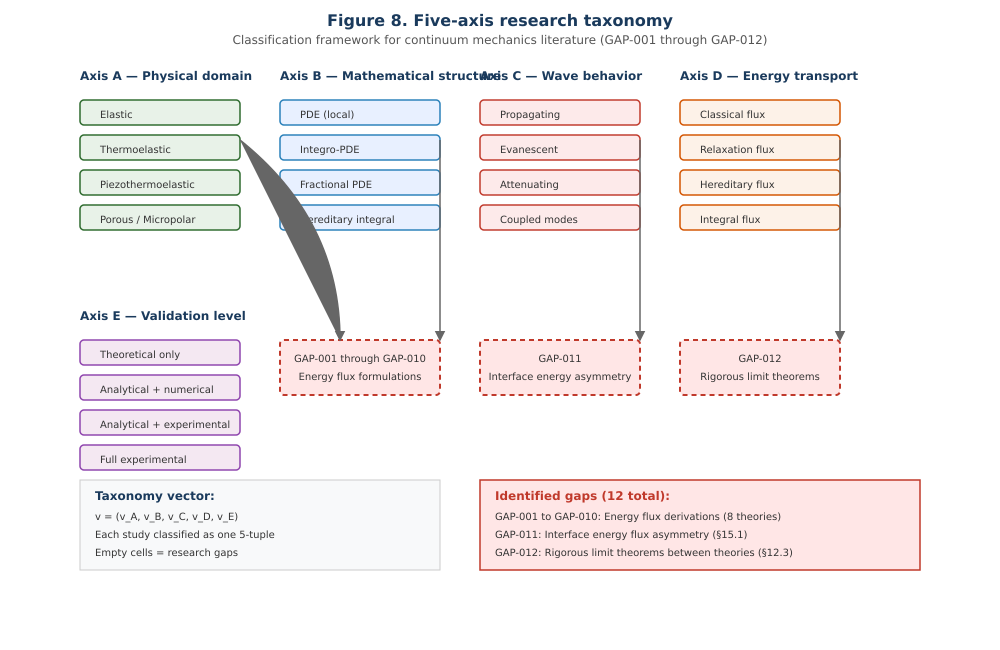
\includegraphics[width=0.9\textwidth]{../figures/source/fig08_taxonomy.svg}
\caption{Five-axis research taxonomy: physical (material type), mathematical (PDE/integral/fractional), wave (P/S/T/coupled), energy (mechanical/thermal/electrical), and validation (theory/analytical/experimental) dimensions. Each study is classified as a vector across all five axes.}
\label{fig:taxonomy}
\end{figure}

\subsection{Five-axis taxonomy}
\label{sec:14.1}

The five-axis taxonomy classifies each study across five independent dimensions:

\begin{enumerate}
\item \textbf{Physical axis:} Material type (elastic, thermoelastic, piezothermoelastic, porous, micropolar, semiconductor, magneto-thermo-elastic).
\item \textbf{Mathematical axis:} Mathematical structure (PDE, integro-PDE, fractional PDE, nonlocal integral, hereditary integral).
\item \textbf{Wave axis:} Wave types supported (P, S, thermal, evanescent, attenuating, coupled modes).
\item \textbf{Energy axis:} Energy transport mechanism (classical flux, relaxation flux, hereditary flux, integral flux, electrical flux).
\item \textbf{Validation axis:} Validation level (theoretical only, analytical + numerical, analytical + experimental, full experimental).
\end{enumerate}

Each axis is further subdivided into categories, producing a multi-dimensional classification space.

\subsection{Application to the evidence base}
\label{sec:14.2}

The taxonomy is applied to the literature database (88 records currently, expanding to 500+). Each study is classified across all five axes, producing a taxonomy vector:

\begin{equation}
\bm{v} = (v_\text{physical}, v_\text{mathematical}, v_\text{wave}, v_\text{energy}, v_\text{validation}).
\label{eq:14.1}
\end{equation}

Studies with similar taxonomy vectors form clusters, revealing research concentrations and gaps.

\subsection{Empty cells: research gaps identified by taxonomy}
\label{sec:14.3}

Empty cells in the taxonomy (combinations with no or few studies) identify research gaps:

\begin{table}[h]
\centering
\small
\caption{Research gaps identified by empty taxonomy cells.}
\label{tab:taxonomy_gaps}
\begin{tabularx}{\textwidth}{@{}lXrX@{}}
\toprule
\textbf{Gap ID} & \textbf{Description} & \textbf{Priority} & \textbf{Related section} \\
\midrule
GAP-001 & Energy flux for LS theory in time domain & High & Section 10.3 \\
GAP-002 & Energy flux for GL theory & High & Section 10.3 \\
GAP-003 & Energy flux for GN-II theory & High & Section 10.3 \\
GAP-004 & Energy flux for GN-III theory & High & Section 10.3 \\
GAP-005 & Energy flux for DPL theory in time domain & High & Section 10.3 \\
GAP-006 & Energy flux for TPL theory & High & Section 10.3 \\
GAP-007 & Energy flux for MGT theory & High & Section 10.3 \\
GAP-008 & MDD hereditary energy flux & High & Section 10.3 \\
GAP-009 & Nonlocal integral-form energy flux & High & Section 10.3 \\
GAP-010 & Piezoelectric electrical energy flux & High & Section 10.3 \\
GAP-011 & Energy flux asymmetry at multiphysics interfaces & High & Section 15.1 \\
GAP-012 & Rigorous limit theorems between theories & Medium & Section 12.3 \\
\bottomrule
\end{tabularx}
\end{table}

GAP-011 (energy flux asymmetry at interfaces) is documented from RG-003 observations, not as an error allegation.

\subsection{Contradiction mapping: pairs of studies with contradictory approaches}
\label{sec:14.4}

Apparent contradictions between studies are mapped to their root causes:

\begin{table}[h]
\centering
\small
\caption{Contradiction mapping framework.}
\label{tab:contradiction_map}
\begin{tabularx}{\textwidth}{@{}lXXX@{}}
\toprule
\textbf{Contradiction type} & \textbf{Root cause} & \textbf{Resolution approach} & \textbf{Example} \\
\midrule
Assumption difference & Different constitutive assumptions & Trace to primary sources & LS vs. GL relaxation mechanism \\
Approximation difference & Different Taylor expansion orders & Compare validity ranges & DPL first-order vs. second-order \\
Normalization difference & Different reference values & Convert to common units & Temperature reference \\
Frequency convention & $e^{i\omega t}$ vs. $e^{-i\omega t}$ & Standardize convention & Sign of imaginary parts \\
\bottomrule
\end{tabularx}
\end{table}

Each contradiction is resolved by tracing to assumptions, not by declaring any study erroneous.

\subsection{Advantages over single-axis classifications}
\label{sec:14.5}

The five-axis taxonomy offers several advantages:

\begin{enumerate}
\item \textbf{Multi-dimensional:} Captures complexity that single-axis classifications miss,
\item \textbf{Gap identification:} Empty cells reveal underexplored research areas,
\item \textbf{Contradiction resolution:} Differences traced to specific assumptions,
\item \textbf{Comparability:} Enables systematic comparison across theory families,
\item \textbf{Extensibility:} New axes can be added as research evolves.
\end{enumerate}

\subsection{Limitations}
\label{sec:14.6}

\begin{enumerate}
\item \textbf{Analyst-constructed:} The taxonomy is constructed by the analyst, not discovered from data,
\item \textbf{Abstract-only classifications:} Many studies are classified from abstracts only, limiting accuracy,
\item \textbf{Subjectivity:} Classification decisions involve analyst judgment,
\item \textbf{Incomplete coverage:} Current database covers 88 records, expanding to 500+.
\end{enumerate}

These limitations are acknowledged; the taxonomy is presented as a research tool, not as a definitive classification.

\subsection{Notation summary for Section 14}

\begin{table}[h]
\centering
\small
\caption{Notation introduced in Section 14.}
\label{tab:notation-sec14}
\begin{tabularx}{\textwidth}{@{}lXlr@{}}
\toprule
\textbf{Symbol} & \textbf{Meaning} & \textbf{Units} & \textbf{Equation} \\
\midrule
$\bm{v}$ & Taxonomy vector & dimensionless & \eqref{eq:14.1} \\
\bottomrule
\end{tabularx}
\end{table}

\subsection{Open questions for Section 14}

\begin{enumerate}[label=\textbf{OQ14.\arabic*}]
\item How can the taxonomy be validated against independent analyst classifications? \label{oq:14.1}
\item What additional axes would improve the taxonomy's coverage? \label{oq:14.2}
\end{enumerate}

% LocalWords: 
